% ============================================================
% 讲义 — 人教版九年级上册 · 第22章 二次函数
% 编译命令：xelatex -interaction=nonstopmode 第22章_二次函数.tex
% ============================================================
\documentclass[12pt, a4paper]{ctexart}
\usepackage[margin=2.2cm]{geometry}
\usepackage{amsmath, amssymb}
\usepackage{enumitem}
\usepackage{tcolorbox}
\usepackage{booktabs}
\usepackage{array}
\usepackage{fancyhdr}
\usepackage{xcolor}
\usepackage{tikz}
\usepackage{hyperref}
\usepackage{graphicx}
\usepackage{multirow}
\usepackage{pgfplots}
\pgfplotsset{compat=1.18}

% 颜色定义
\definecolor{mainblue}{RGB}{41, 98, 168}
\definecolor{lightblue}{RGB}{230, 240, 255}
\definecolor{tipgreen}{RGB}{34, 139, 87}
\definecolor{lightgreen}{RGB}{235, 250, 240}
\definecolor{warnred}{RGB}{200, 50, 50}
\definecolor{lightred}{RGB}{255, 240, 240}
\definecolor{examorange}{RGB}{210, 120, 20}
\definecolor{lightorange}{RGB}{255, 248, 235}
\definecolor{apppurple}{RGB}{120, 60, 170}
\definecolor{lightpurple}{RGB}{245, 238, 255}

% 页眉页脚
\pagestyle{fancy}
\fancyhf{}
\fancyhead[L]{\small\textcolor{mainblue}{\textbf{人教版九年级上册 · 第22章 二次函数}}}
\fancyhead[R]{\small\textcolor{mainblue}{家教讲义}}
\fancyfoot[C]{\small —\ \thepage\ —}
\renewcommand{\headrulewidth}{0.6pt}
\renewcommand{\headrule}{\hbox to\headwidth{\color{mainblue}\leaders\hrule height \headrulewidth\hfill}}
\renewcommand{\footrulewidth}{0pt}

% tcolorbox 样式
\newtcolorbox{knowledgebox}[1][]{%
  colback=lightblue, colframe=mainblue,
  fonttitle=\bfseries\large, title=#1,
  arc=3mm, boxrule=0.8pt,
  left=8pt, right=8pt, top=6pt, bottom=6pt
}

\newtcolorbox{tipbox}[1][]{%
  colback=lightgreen, colframe=tipgreen,
  fonttitle=\bfseries, title=#1,
  arc=2mm, boxrule=0.6pt,
  left=6pt, right=6pt, top=4pt, bottom=4pt
}

\newtcolorbox{warnbox}[1][]{%
  colback=lightred, colframe=warnred,
  fonttitle=\bfseries, title=#1,
  arc=2mm, boxrule=0.6pt,
  left=6pt, right=6pt, top=4pt, bottom=4pt
}

\newtcolorbox{examplebox}[1][]{%
  colback=lightorange, colframe=examorange,
  fonttitle=\bfseries, title=#1,
  arc=3mm, boxrule=0.8pt,
  left=8pt, right=8pt, top=6pt, bottom=6pt
}

\newtcolorbox{appbox}[1][]{%
  colback=lightpurple, colframe=apppurple,
  fonttitle=\bfseries, title=#1,
  arc=3mm, boxrule=0.8pt,
  left=8pt, right=8pt, top=6pt, bottom=6pt
}

\setCJKmainfont{Hiragino Sans GB}
\setCJKsansfont{Heiti SC}

\begin{document}

% ============ 标题页 ============
\begin{center}
{\Huge\bfseries\textcolor{mainblue}{第22章\quad 二次函数}}\\[12pt]
{\Large\textcolor{gray}{家\quad 教\quad 讲\quad 义}}\\[8pt]
\rule{0.6\textwidth}{1pt}\\[8pt]
{\normalsize 适用：人教版九年级上册\quad |\quad 课时：8$\sim$10课时}
\end{center}
\vspace{10pt}

% ============================================================
% 第一部分：知识点讲解
% ============================================================
\section*{\textcolor{mainblue}{一、知识点讲解}}

\subsection*{22.1\quad 二次函数的概念与三种形式}

\begin{knowledgebox}[二次函数的定义]
一般地，形如
\[
\boxed{y = ax^2 + bx + c \quad (a \neq 0)}
\]
的函数叫做二次函数，其中 $x$ 是自变量，$a$、$b$、$c$ 是常数，且 $a \neq 0$。
\end{knowledgebox}

\begin{knowledgebox}[二次函数的三种表达形式]
\textbf{（1）一般式：}
\[
y = ax^2 + bx + c
\]
可以直观地读出 $c$ 为 $y$ 轴截距（即图象过点 $(0,c)$）。

\medskip
\textbf{（2）顶点式：}
\[
\boxed{y = a(x-h)^2 + k}
\]
顶点坐标为 $(h,\,k)$，对称轴为 $x=h$。由一般式配方可得：
\[
h = -\frac{b}{2a}, \qquad k = \frac{4ac - b^2}{4a} = c - \frac{b^2}{4a}
\]

\medskip
\textbf{（3）交点式（两根式）：}
\[
y = a(x - x_1)(x - x_2)
\]
其中 $x_1$、$x_2$ 是抛物线与 $x$ 轴的两个交点的横坐标（即方程 $ax^2+bx+c=0$ 的两个根）。当 $\Delta < 0$ 时，此形式不适用。
\end{knowledgebox}

\subsection*{22.2\quad 抛物线的基本性质}

\begin{knowledgebox}[抛物线 $y=ax^2+bx+c$ 的性质]
\begin{enumerate}[leftmargin=*]
  \item \textbf{开口方向}：$a > 0$ 时开口向上；$a < 0$ 时开口向下。$|a|$ 越大，开口越小。
  \item \textbf{对称轴}：直线 $\displaystyle x = -\frac{b}{2a}$。
  \item \textbf{顶点坐标}：$\displaystyle\left(-\frac{b}{2a},\;\frac{4ac-b^2}{4a}\right)$。
  \item \textbf{与 $y$ 轴的交点}：$(0,\,c)$。
  \item \textbf{与 $x$ 轴的交点}：由 $\Delta = b^2-4ac$ 决定。
  \begin{itemize}
    \item $\Delta > 0$：与 $x$ 轴有两个交点 $\left(\dfrac{-b \pm \sqrt{\Delta}}{2a},\; 0\right)$。
    \item $\Delta = 0$：与 $x$ 轴有一个交点（顶点在 $x$ 轴上）。
    \item $\Delta < 0$：与 $x$ 轴没有交点。
  \end{itemize}
\end{enumerate}
\end{knowledgebox}

\begin{center}
\begin{tikzpicture}
\begin{axis}[
  axis lines=middle,
  xlabel={$x$}, ylabel={$y$},
  xmin=-3.5, xmax=4.5, ymin=-4, ymax=6,
  width=10cm, height=7cm,
  xtick={-3,-2,-1,0,1,2,3,4},
  ytick={-4,-3,-2,-1,0,1,2,3,4,5},
  grid=major,
  grid style={dashed, gray!30},
  every axis x label/.style={at={(ticklabel* cs:1)},anchor=west},
  every axis y label/.style={at={(ticklabel* cs:1)},anchor=south},
]
% 抛物线 y = x^2 - 2x - 3 = (x-1)^2 - 4，顶点(1,-4)
\addplot[blue, thick, domain=-2.5:4.5, samples=100] {x^2 - 2*x - 3};
% 顶点
\node[fill=red, circle, inner sep=2pt] at (axis cs:1,-4) {};
\node[above right] at (axis cs:1,-4) {\small 顶点$(1,-4)$};
% 对称轴
\addplot[dashed, red, domain=-4:6] coordinates {(1,-4.5) (1,6)};
\node[above] at (axis cs:1,5.5) {\small 对称轴 $x=1$};
% 与x轴交点
\node[fill=blue, circle, inner sep=2pt] at (axis cs:-1,0) {};
\node[below left] at (axis cs:-1,0) {\small $(-1,0)$};
\node[fill=blue, circle, inner sep=2pt] at (axis cs:3,0) {};
\node[below right] at (axis cs:3,0) {\small $(3,0)$};
% 与y轴交点
\node[fill=blue, circle, inner sep=2pt] at (axis cs:0,-3) {};
\node[left] at (axis cs:0,-3) {\small $(0,-3)$};
\end{axis}
\end{tikzpicture}
\end{center}

\begin{warnbox}[重点：$a$、$b$、$c$ 的符号与图象特征]
\begin{enumerate}[leftmargin=*]
  \item \textbf{$a$ 的符号}：$a>0$ 开口向上；$a<0$ 开口向下。
  \item \textbf{$c$ 的符号}：$c>0$ 时抛物线与 $y$ 轴交于正半轴；$c<0$ 交于负半轴；$c=0$ 过原点。
  \item \textbf{$b$ 的符号}：对称轴 $x=-\dfrac{b}{2a}$，结合 $a$ 的符号判断。
  \begin{itemize}
    \item 若 $a$、$b$ 同号（$ab>0$），则对称轴在 $y$ 轴\textbf{左侧}。
    \item 若 $a$、$b$ 异号（$ab<0$），则对称轴在 $y$ 轴\textbf{右侧}。
    \item 若 $b=0$，则对称轴为 $y$ 轴。
  \end{itemize}
  \item \textbf{$b^2-4ac$（即 $\Delta$）的符号}：$\Delta>0$ 与 $x$ 轴有两个交点；$\Delta=0$ 与 $x$ 轴相切；$\Delta<0$ 与 $x$ 轴无交点。
  \item \textbf{特殊点}：令 $x=1$，$y=a+b+c$；令 $x=-1$，$y=a-b+c$。由图象上 $x=\pm 1$ 处的函数值可判断 $a+b+c$ 和 $a-b+c$ 的符号。
\end{enumerate}
\end{warnbox}

\begin{center}
\begin{tikzpicture}
% 展示 a>0 和 a<0 两种情况的对比
\begin{axis}[
  axis lines=middle,
  xlabel={$x$}, ylabel={$y$},
  xmin=-4, xmax=4, ymin=-5, ymax=5,
  width=7cm, height=5.5cm,
  xtick=\empty, ytick=\empty,
  grid=major,
  grid style={dashed, gray!20},
  title={\small $a>0$，开口向上},
  title style={at={(0.5,1.05)}},
]
\addplot[blue, thick, domain=-3:3, samples=80] {0.8*(x-1)^2 - 3};
\node[fill=red, circle, inner sep=1.5pt] at (axis cs:1,-3) {};
\end{axis}
\end{tikzpicture}
\hspace{1cm}
\begin{tikzpicture}
\begin{axis}[
  axis lines=middle,
  xlabel={$x$}, ylabel={$y$},
  xmin=-4, xmax=4, ymin=-5, ymax=5,
  width=7cm, height=5.5cm,
  xtick=\empty, ytick=\empty,
  grid=major,
  grid style={dashed, gray!20},
  title={\small $a<0$，开口向下},
  title style={at={(0.5,1.05)}},
]
\addplot[blue, thick, domain=-3:3, samples=80] {-0.8*(x+1)^2 + 3};
\node[fill=red, circle, inner sep=1.5pt] at (axis cs:-1,3) {};
\end{axis}
\end{tikzpicture}
\end{center}

\subsection*{22.3\quad 二次函数与一元二次方程的关系}

\begin{knowledgebox}[二次函数与方程的关系]
二次函数 $y = ax^2+bx+c$ 的图象与 $x$ 轴交点的横坐标，就是一元二次方程 $ax^2+bx+c=0$ 的根。
\medskip
\begin{tabular}{l|l|l}
\toprule
$\Delta$ 的符号 & 方程的根 & 图象与 $x$ 轴的关系 \\
\midrule
$\Delta > 0$ & 两个不等实根 $x_1,\;x_2$ & 两个交点 $(x_1,0)$、$(x_2,0)$ \\
$\Delta = 0$ & 两个相等实根 $x_1=x_2$ & 一个交点（相切） \\
$\Delta < 0$ & 无实根 & 无交点 \\
\bottomrule
\end{tabular}
\end{knowledgebox}

\subsection*{22.4\quad 二次函数的最值}

\begin{knowledgebox}[二次函数的最值]
对于 $y = a(x-h)^2+k$：
\begin{itemize}[leftmargin=*]
  \item 当 $a > 0$ 时，$x=h$ 时 $y$ 取\textbf{最小值} $k$，无最大值。
  \item 当 $a < 0$ 时，$x=h$ 时 $y$ 取\textbf{最大值} $k$，无最小值。
\end{itemize}
\medskip
如果限制了自变量的取值范围 $[m,\,n]$，则需要比较端点值和顶点值：
\begin{enumerate}[leftmargin=*]
  \item 若顶点横坐标 $h \in [m,n]$，则最值在顶点和两个端点中取。
  \item 若 $h \notin [m,n]$，则最值在端点处取得。
\end{enumerate}
\end{knowledgebox}

\begin{tipbox}[求最值的方法总结]
\begin{enumerate}[leftmargin=*]
  \item \textbf{顶点式法}：配方后直接读出最值。
  \item \textbf{公式法}：最值 $y_{\text{极}} = \dfrac{4ac-b^2}{4a}$，在 $x=-\dfrac{b}{2a}$ 处取得。
  \item \textbf{限定范围}：画出草图，结合单调性判断。
\end{enumerate}
\end{tipbox}

% ============================================================
% 第二部分：例题精讲
% ============================================================
\section*{\textcolor{examorange}{二、例题精讲}}

\begin{examplebox}[【例1】由一般式写成顶点式，并画图]
将 $y = 2x^2 - 8x + 6$ 化为顶点式，写出顶点坐标、对称轴，并画出函数图象。
\end{examplebox}

\textbf{解：}

配方：
\[
y = 2x^2 - 8x + 6 = 2(x^2 - 4x) + 6 = 2(x^2 - 4x + 4 - 4) + 6 = 2(x-2)^2 - 2
\]
所以顶点式为 $y = 2(x-2)^2 - 2$。

顶点坐标为 $(2,\,-2)$，对称轴为 $x=2$，开口向上。

\begin{center}
\begin{tikzpicture}
\begin{axis}[
  axis lines=middle,
  xlabel={$x$}, ylabel={$y$},
  xmin=-0.5, xmax=4.5, ymin=-3, ymax=8,
  width=9cm, height=6cm,
  xtick={0,1,2,3,4},
  ytick={-2,0,2,4,6,8},
  grid=major,
  grid style={dashed, gray!30},
  every axis x label/.style={at={(ticklabel* cs:1)},anchor=west},
  every axis y label/.style={at={(ticklabel* cs:1)},anchor=south},
]
\addplot[blue, thick, domain=-0.2:4.2, samples=80] {2*(x-2)^2 - 2};
\node[fill=red, circle, inner sep=2pt] at (axis cs:2,-2) {};
\node[right] at (axis cs:2,-2) {\small 顶点$(2,-2)$};
\addplot[dashed, red, domain=-3:9] coordinates {(2,-3.5) (2,8.5)};
\node[above] at (axis cs:2,8) {\small $x=2$};
\node[fill=blue, circle, inner sep=1.5pt] at (axis cs:1,0) {};
\node[below left] at (axis cs:1,0) {\small $(1,0)$};
\node[fill=blue, circle, inner sep=1.5pt] at (axis cs:3,0) {};
\node[below right] at (axis cs:3,0) {\small $(3,0)$};
\node[fill=blue, circle, inner sep=1.5pt] at (axis cs:0,6) {};
\node[above left] at (axis cs:0,6) {\small $(0,6)$};
\end{axis}
\end{tikzpicture}
\end{center}

与 $x$ 轴的交点：令 $2(x-2)^2-2=0$，$(x-2)^2=1$，$x=1$ 或 $x=3$，交点为 $(1,0)$ 和 $(3,0)$。

与 $y$ 轴的交点：令 $x=0$，$y=6$，交点为 $(0,6)$。

\begin{examplebox}[【例2】由已知条件求二次函数]
已知二次函数的图象经过点 $A(-1,0)$、$B(3,0)$ 和 $C(0,-3)$，求这个二次函数的解析式。
\end{examplebox}

\textbf{解：}

\textbf{方法一（交点式）：}

因为图象过 $A(-1,0)$ 和 $B(3,0)$，设交点式：
\[
y = a(x+1)(x-3)
\]
代入 $C(0,-3)$：$-3 = a \cdot 1 \cdot (-3) = -3a$，所以 $a=1$。

解析式为 $\boxed{y = (x+1)(x-3) = x^2 - 2x - 3}$。

\textbf{方法二（一般式）：}

设 $y = ax^2+bx+c$，代入三点坐标列方程组：
\[
\begin{cases}
a - b + c = 0 \\
9a + 3b + c = 0 \\
c = -3
\end{cases}
\]
由第三个方程 $c=-3$，代入前两个得：
\[
\begin{cases}
a - b = 3 \\
9a + 3b = 3
\end{cases}
\]
解得 $a=1$，$b=-2$，所以 $y = x^2 - 2x - 3$。

\begin{examplebox}[【例3】$a$、$b$、$c$ 的符号判断]
已知二次函数 $y=ax^2+bx+c$ 的图象如图所示，下列结论正确的是\quad（\quad）

\begin{center}
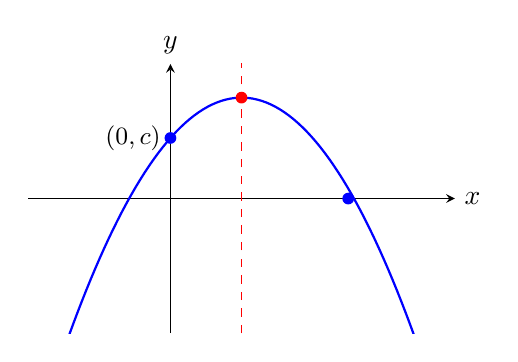
\begin{tikzpicture}
\begin{axis}[
  axis lines=middle,
  xlabel={$x$}, ylabel={$y$},
  xmin=-2, xmax=4, ymin=-4, ymax=4,
  width=7cm, height=5cm,
  xtick=\empty, ytick=\empty,
  every axis x label/.style={at={(ticklabel* cs:1)},anchor=west},
  every axis y label/.style={at={(ticklabel* cs:1)},anchor=south},
]
\addplot[blue, thick, domain=-1.5:3.5, samples=80] {-1.2*(x-1)^2 + 3};
\node[fill=red, circle, inner sep=1.5pt] at (axis cs:1,3) {};
\addplot[dashed, red, domain=-4:4] coordinates {(1,-4.5) (1,4.5)};
\node[fill=blue, circle, inner sep=1.5pt] at (axis cs:0,1.8) {};
\node[left] at (axis cs:0,1.8) {\small $(0,c)$};
\node[fill=blue, circle, inner sep=1.5pt] at (axis cs:2.5,0) {};
\end{axis}
\end{tikzpicture}
\end{center}

(A) $a>0,\; b>0,\; c>0$\quad
(B) $a<0,\; b>0,\; c>0$

(C) $a<0,\; b<0,\; c>0$\quad
(D) $a<0,\; b>0,\; c<0$
\end{examplebox}

\textbf{解：}

由图象：
\begin{itemize}[leftmargin=*]
  \item 开口向下 $\implies a < 0$。
  \item 对称轴在 $y$ 轴右侧（$x=1>0$），即 $-\dfrac{b}{2a} > 0$。因为 $a<0$，所以 $\dfrac{b}{2|a|} > 0$，即 $b > 0$。
  \item 与 $y$ 轴交于正半轴 $\implies c > 0$。
\end{itemize}

所以 $a<0$，$b>0$，$c>0$，选 \textbf{(B)}。

\begin{warnbox}[判断技巧：口诀]
\begin{itemize}[leftmargin=*]
  \item "$a$ 看开口"：上正下负。
  \item "$b$ 看对称轴"：左同右异（对称轴在 $y$ 轴左边，则 $a$、$b$ 同号；右边则异号）。
  \item "$c$ 看截距"：上正下负（与 $y$ 轴交点在正半轴则 $c>0$）。
\end{itemize}
\end{warnbox}

\begin{examplebox}[【例4】二次函数与方程的关系]
已知二次函数 $y = x^2 - 2x - 3$。
\begin{enumerate}[leftmargin=*]
  \item 求图象与 $x$ 轴的交点坐标。
  \item 当 $x$ 取何值时，$y > 0$？$y < 0$？
\end{enumerate}
\end{examplebox}

\textbf{解：}

令 $y=0$：$x^2-2x-3=0$，$(x-3)(x+1)=0$，$x_1=-1$，$x_2=3$。

(1) 与 $x$ 轴的交点为 $(-1,\,0)$ 和 $(3,\,0)$。

(2) 因为 $a=1>0$（开口向上），所以：
\begin{itemize}[leftmargin=*]
  \item $y > 0$ 时：$x < -1$ 或 $x > 3$。
  \item $y < 0$ 时：$-1 < x < 3$。
  \item $y = 0$ 时：$x = -1$ 或 $x = 3$。
\end{itemize}

\begin{center}
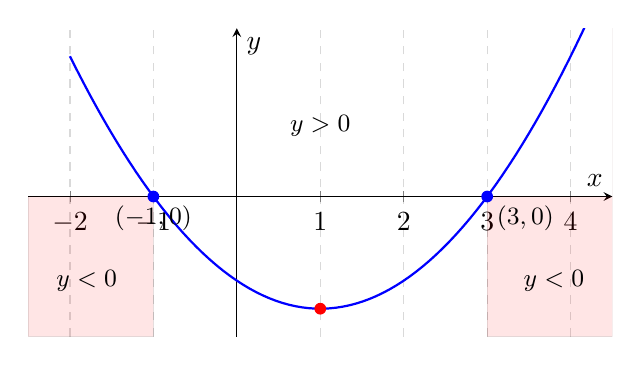
\begin{tikzpicture}
\begin{axis}[
  axis lines=middle,
  xlabel={$x$}, ylabel={$y$},
  xmin=-2.5, xmax=4.5, ymin=-5, ymax=6,
  width=9cm, height=5.5cm,
  xtick={-2,-1,0,1,2,3,4},
  ytick=\empty,
  grid=major,
  grid style={dashed, gray!30},
]
\addplot[blue, thick, domain=-2:4.3, samples=80] {x^2 - 2*x - 3};
% 阴影区域
\addplot[fill=red, opacity=0.1] coordinates {(-2.5,-5) (-1,-5) (-1,0)} \closedcycle;
\addplot[fill=red, opacity=0.1] coordinates {(3,0) (3,-5) (4.5,-5) (4.5,6)} \closedcycle;
\node at (axis cs:-1.8,-3) {\small $y<0$};
\node at (axis cs:3.8,-3) {\small $y<0$};
\node at (axis cs:1,2.5) {\small $y>0$};
\node[fill=blue, circle, inner sep=1.5pt] at (axis cs:-1,0) {};
\node[below] at (axis cs:-1,0) {\small $(-1,0)$};
\node[fill=blue, circle, inner sep=1.5pt] at (axis cs:3,0) {};
\node[below right] at (axis cs:3,0) {\small $(3,0)$};
\node[fill=red, circle, inner sep=1.5pt] at (axis cs:1,-4) {};
\end{axis}
\end{tikzpicture}
\end{center}

\begin{examplebox}[【例5】二次函数的最值]
求函数 $y = -x^2 + 4x - 1$ 的最大值，并求取得最大值时 $x$ 的值。
\end{examplebox}

\textbf{解：}

方法一（配方法）：
\[
y = -x^2 + 4x - 1 = -(x^2 - 4x) - 1 = -(x^2 - 4x + 4 - 4) - 1 = -(x-2)^2 + 3
\]
因为 $a = -1 < 0$，所以当 $x = 2$ 时，$y$ 取最大值 $\boxed{y_{\max} = 3}$。

方法二（公式法）：
\[
x = -\frac{b}{2a} = -\frac{4}{2\times(-1)} = 2
\]
\[
y_{\max} = \frac{4ac - b^2}{4a} = \frac{4\times(-1)\times(-1) - 16}{4\times(-1)} = \frac{4-16}{-4} = \frac{-12}{-4} = 3
\]

\begin{examplebox}[【例6】限定范围的最值问题]
当 $0 \leqslant x \leqslant 3$ 时，求函数 $y = x^2 - 2x + 3$ 的最大值和最小值。
\end{examplebox}

\textbf{解：}

配方：$y = (x-1)^2 + 2$，顶点为 $(1,\,2)$，$a=1>0$ 开口向上。

顶点横坐标 $x=1 \in [0,\,3]$，所以最小值在顶点处取得：$y_{\min} = 2$。

最大值在端点处取得，比较两个端点：
\begin{itemize}[leftmargin=*]
  \item $x=0$ 时，$y = 0-0+3 = 3$。
  \item $x=3$ 时，$y = 9-6+3 = 6$。
\end{itemize}

所以 $y_{\max} = 6$（当 $x=3$ 时）。

\textbf{答：}最小值为 $\boxed{2}$（$x=1$ 时），最大值为 $\boxed{6}$（$x=3$ 时）。

\begin{center}
\begin{tikzpicture}
\begin{axis}[
  axis lines=middle,
  xlabel={$x$}, ylabel={$y$},
  xmin=-0.5, xmax=3.5, ymin=0, ymax=7,
  width=8cm, height=5.5cm,
  xtick={0,1,2,3},
  ytick={0,1,2,3,4,5,6},
  grid=major,
  grid style={dashed, gray!30},
  extra x ticks={0,3},
  extra x tick style={grid=major, grid style={thick, red, dashed}},
]
\addplot[blue, thick, domain=-0.2:3.2, samples=80] {x^2 - 2*x + 3};
\node[fill=red, circle, inner sep=2pt] at (axis cs:1,2) {};
\node[below right] at (axis cs:1,2) {\small 最小值$(1,2)$};
\node[fill=red, circle, inner sep=2pt] at (axis cs:3,6) {};
\node[above right] at (axis cs:3,6) {\small 最大值$(3,6)$};
\node[fill=blue, circle, inner sep=1.5pt] at (axis cs:0,3) {};
\node[above left] at (axis cs:0,3) {\small $(0,3)$};
\end{axis}
\end{tikzpicture}
\end{center}

\begin{examplebox}[【例7】抛物线的平移]
将抛物线 $y = 2x^2$ 先向右平移 $3$ 个单位，再向下平移 $2$ 个单位，求平移后抛物线的解析式。
\end{examplebox}

\textbf{解：}

向右平移 $3$ 个单位：$y = 2x^2 \to y = 2(x-3)^2$。

再向下平移 $2$ 个单位：$y = 2(x-3)^2 \to y = 2(x-3)^2 - 2$。

所以平移后的解析式为 $\boxed{y = 2(x-3)^2 - 2}$。

展开验证：$y = 2(x^2-6x+9) - 2 = 2x^2 - 12x + 16$。

\begin{tipbox}[平移口诀]
"左加右减，上加下减"。$y=a(x-h)^2+k$ 中，$h$ 控制左右平移，$k$ 控制上下平移。
\end{tipbox}

\begin{examplebox}[【例8】综合题：二次函数与几何]
已知抛物线 $y = x^2 - 2x - 3$ 与 $x$ 轴交于 $A$、$B$ 两点（$A$ 在 $B$ 左侧），顶点为 $C$。求 $\triangle ABC$ 的面积。
\end{examplebox}

\textbf{解：}

令 $y=0$：$x^2-2x-3=0$，$(x-3)(x+1)=0$，$A(-1,0)$，$B(3,0)$。

配方：$y=(x-1)^2-4$，顶点 $C(1,-4)$。

$AB = |3-(-1)| = 4$。

$C$ 到 $x$ 轴的距离（即 $\triangle ABC$ 的高）$h = |-4| = 4$。

$S_{\triangle ABC} = \dfrac{1}{2} \times AB \times h = \dfrac{1}{2} \times 4 \times 4 = \boxed{8}$。

% ============================================================
% 第三部分：应用题
% ============================================================
\section*{\textcolor{apppurple}{三、应用题}}

\begin{appbox}[【应用1】抛物线型拱桥]
一座拱桥的桥拱是抛物线形，桥拱的跨度为 $20$\,m，拱高为 $4$\,m。在拱桥下方的水面宽为 $12$\,m 时，水面距桥拱顶部有多远？
\end{appbox}

\textbf{解：}

以拱桥底部水平线的中点为原点，向上为 $y$ 轴正方向建立坐标系。则拱顶坐标为 $(0,4)$，拱桥两端为 $(-10,0)$ 和 $(10,0)$。

设抛物线方程为 $y = ax^2 + 4$。

代入 $(10,0)$：$0 = 100a + 4$，$a = -\dfrac{1}{25}$。

所以 $y = -\dfrac{1}{25}x^2 + 4$。

水面宽 $12$\,m 时，$x = \pm 6$。代入：
\[
y = -\frac{1}{25} \times 36 + 4 = -\frac{36}{25} + 4 = \frac{-36+100}{25} = \frac{64}{25} = 2.56
\]
水面距拱顶的距离为 $4 - 2.56 = 1.44$\,m。

\textbf{答：}水面距桥拱顶部有 $\boxed{1.44}$\,m。

\begin{center}
\begin{tikzpicture}
\begin{axis}[
  axis lines=middle,
  xlabel={$x$（米）}, ylabel={$y$（米）},
  xmin=-12, xmax=12, ymin=-1, ymax=5,
  width=10cm, height=5.5cm,
  xtick={-10,-8,-6,-4,-2,0,2,4,6,8,10},
  ytick={0,1,2,2.56,3,4},
  grid=major,
  grid style={dashed, gray!20},
  every axis x label/.style={at={(ticklabel* cs:1)},anchor=west},
  every axis y label/.style={at={(ticklabel* cs:1)},anchor=south},
]
\addplot[blue, thick, domain=-10:10, samples=80] {-1/25*x^2 + 4};
% 标注
\node[fill=red, circle, inner sep=1.5pt] at (axis cs:0,4) {};
\node[above] at (axis cs:0,4) {\small 拱顶$(0,4)$};
\node[fill=blue, circle, inner sep=1.5pt] at (axis cs:-10,0) {};
\node[below] at (axis cs:-10,0) {\small $(-10,0)$};
\node[fill=blue, circle, inner sep=1.5pt] at (axis cs:10,0) {};
\node[below] at (axis cs:10,0) {\small $(10,0)$};
\node[fill=blue, circle, inner sep=1.5pt] at (axis cs:-6,2.56) {};
\node[left] at (axis cs:-6,2.56) {\small $(-6,2.56)$};
\node[fill=blue, circle, inner sep=1.5pt] at (axis cs:6,2.56) {};
\node[right] at (axis cs:6,2.56) {\small $(6,2.56)$};
% 水面线
\addplot[dashed, red, domain=-6.5:6.5] coordinates {(-6.3,2.56) (6.3,2.56)};
\node[right, red] at (axis cs:7,2.56) {\small 水面};
\end{axis}
\end{tikzpicture}
\end{center}

\begin{appbox}[【应用2】利润最大化]
某公司生产一种产品，年固定成本为 $20$ 万元，每生产 $x$（百件）的总成本函数为 $C(x) = x^2 + 4x + 20$（万元），总收益函数为 $R(x) = -x^2 + 24x$（万元）。问：年产量为多少百件时，公司获得的利润最大？最大利润是多少？
\end{appbox}

\textbf{解：}

利润 $L(x) = R(x) - C(x) = (-x^2+24x) - (x^2+4x+20) = -2x^2 + 20x - 20$。

配方：$L(x) = -2(x^2-10x) - 20 = -2(x^2-10x+25) + 50 - 20 = -2(x-5)^2 + 30$。

因为 $a=-2<0$，所以当 $x=5$（百件）$=500$ 件时，利润取最大值。

$L_{\max} = 30$（万元）。

\textbf{答：}年产量为 $\boxed{500}$ 件时利润最大，最大利润为 $\boxed{30}$ 万元。

\begin{appbox}[【应用3】面积最值]
用总长为 $60$\,m 的篱笆围成一个一边靠墙的矩形花园（墙长足够长），设垂直于墙的一边长为 $x$\,m。
\begin{enumerate}[leftmargin=*]
  \item 写出花园面积 $S$ 与 $x$ 的函数关系式。
  \item 当 $x$ 为多少时，花园面积最大？最大面积是多少？
\end{enumerate}
\end{appbox}

\textbf{解：}

(1) 垂直于墙的一边为 $x$\,m，共两段，则平行于墙的一边为 $(60-2x)$\,m。

面积 $S = x(60-2x) = -2x^2 + 60x$。

其中 $x > 0$ 且 $60-2x > 0$，即 $0 < x < 30$。

(2) 配方：$S = -2(x^2-30x) = -2(x^2-30x+225) + 450 = -2(x-15)^2 + 450$。

当 $x=15$ 时，$S$ 取最大值 $450$\,m$^2$。

此时平行于墙的一边为 $60-2\times15 = 30$\,m。

\textbf{答：}当 $x=\boxed{15}$\,m 时花园面积最大，最大面积为 $\boxed{450}$\,m$^2$。

% ============================================================
% 第四部分：课堂练习 + 参考答案
% ============================================================
\section*{\textcolor{tipgreen}{四、课堂练习}}

\begin{enumerate}[leftmargin=*, label=\textbf{\arabic*.}]
  \item 将 $y = -x^2 + 6x - 5$ 化为顶点式，写出顶点坐标和对称轴。

  \item 已知二次函数的图象经过 $(0,1)$、$(1,0)$、$(-1,4)$ 三点，求函数解析式。

  \item 根据图象判断 $a$、$b$、$c$ 及 $b^2-4ac$ 的符号：

  \begin{center}
  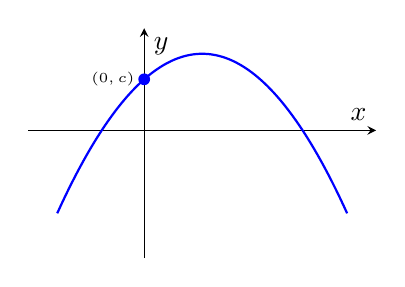
\begin{tikzpicture}
  \begin{axis}[
    axis lines=middle,
    xlabel={$x$}, ylabel={$y$},
    xmin=-2, xmax=4, ymin=-5, ymax=4,
    width=6cm, height=4.5cm,
    xtick=\empty, ytick=\empty,
  ]
  \addplot[blue, thick, domain=-1.5:3.5, samples=80] {-(x-1)^2+3};
  \node[fill=blue, circle, inner sep=1.5pt] at (axis cs:0,2) {};
  \node[left] at (axis cs:0,2) {\tiny $(0,c)$};
  \end{axis}
  \end{tikzpicture}
  \end{center}

  \item 求函数 $y = 2x^2 - 4x + 5$ 在 $-1 \leqslant x \leqslant 4$ 上的最大值和最小值。

  \item 已知抛物线 $y = x^2 - 4x + 3$ 与 $x$ 轴交于 $A$、$B$ 两点，顶点为 $C$，求 $\triangle ABC$ 的面积。

  \item 某商品的利润 $y$（元）与售价 $x$（元）满足关系 $y = -10x^2 + 1000x - 20000$，求利润最大时的售价。
\end{enumerate}

\vspace{6pt}
\begin{knowledgebox}[参考答案]
\textbf{1.}\quad $y = -(x^2-6x) - 5 = -(x^2-6x+9) + 9 - 5 = -(x-3)^2 + 4$。

顶点 $(3,\,4)$，对称轴 $x=3$。

\medskip
\textbf{2.}\quad 设 $y=ax^2+bx+c$。代入 $(0,1)$ 得 $c=1$。代入 $(1,0)$ 得 $a+b+1=0$，即 $a+b=-1$。代入 $(-1,4)$ 得 $a-b+1=4$，即 $a-b=3$。

解方程组：$a=1$，$b=-2$。所以 $\boxed{y = x^2 - 2x + 1 = (x-1)^2}$。

\medskip
\textbf{3.}\quad 开口向下 $\Rightarrow a<0$；对称轴 $x=1>0$，由 $a<0$ 知 $-\dfrac{b}{2a}=1>0 \Rightarrow b>0$；与 $y$ 轴交于正半轴 $\Rightarrow c>0$；与 $x$ 轴有两个交点 $\Rightarrow \Delta = b^2-4ac > 0$。

综上：$a<0,\; b>0,\; c>0,\; b^2-4ac>0$。

\medskip
\textbf{4.}\quad $y=2(x-1)^2+3$，顶点 $(1,3)$，$a>0$ 开口向上。

$x=1 \in [-1,4]$，所以 $y_{\min}=3$（$x=1$ 时）。

$x=-1$ 时 $y=2\times4+3=11$；$x=4$ 时 $y=2\times9+3=21$。

$y_{\max}=21$（$x=4$ 时）。

\medskip
\textbf{5.}\quad $y=(x-2)^2-1$，顶点 $C(2,-1)$。令 $y=0$：$(x-1)(x-3)=0$，$A(1,0)$，$B(3,0)$。

$AB=2$，高 $h=|-1|=1$。$S_{\triangle ABC}=\dfrac{1}{2}\times 2\times 1 = \boxed{1}$。

\medskip
\textbf{6.}\quad $y=-10(x^2-100x)-20000 = -10(x^2-100x+2500)+25000-20000 = -10(x-50)^2+5000$。

当售价 $x=50$ 元时利润最大，最大利润为 $5000$ 元。
\end{knowledgebox}

\vfill
\begin{center}
\small\textcolor{gray}{本讲义仅供教学参考，例题可根据学生水平调整难度。}
\end{center}

\end{document}
